\chapter{Выполнение задания}

\section{Реализуемый алгоритм}
Расчет значения полинома по схеме Горнера.

\section{Выбор языка программирования}
Для выполнения домашнего задания был выбран язык \texttt{C++}.

\section{Код программы}

\lstinputlisting[label=lst:std, caption=Реализация алгоритма расчета значения полинома по схеме Горнера, firstline=11,lastline=36]{../code/main.cpp}

\section{Модели программ}

\subsection{Граф управления программы}

\begin{figure}[h]
	\centering
	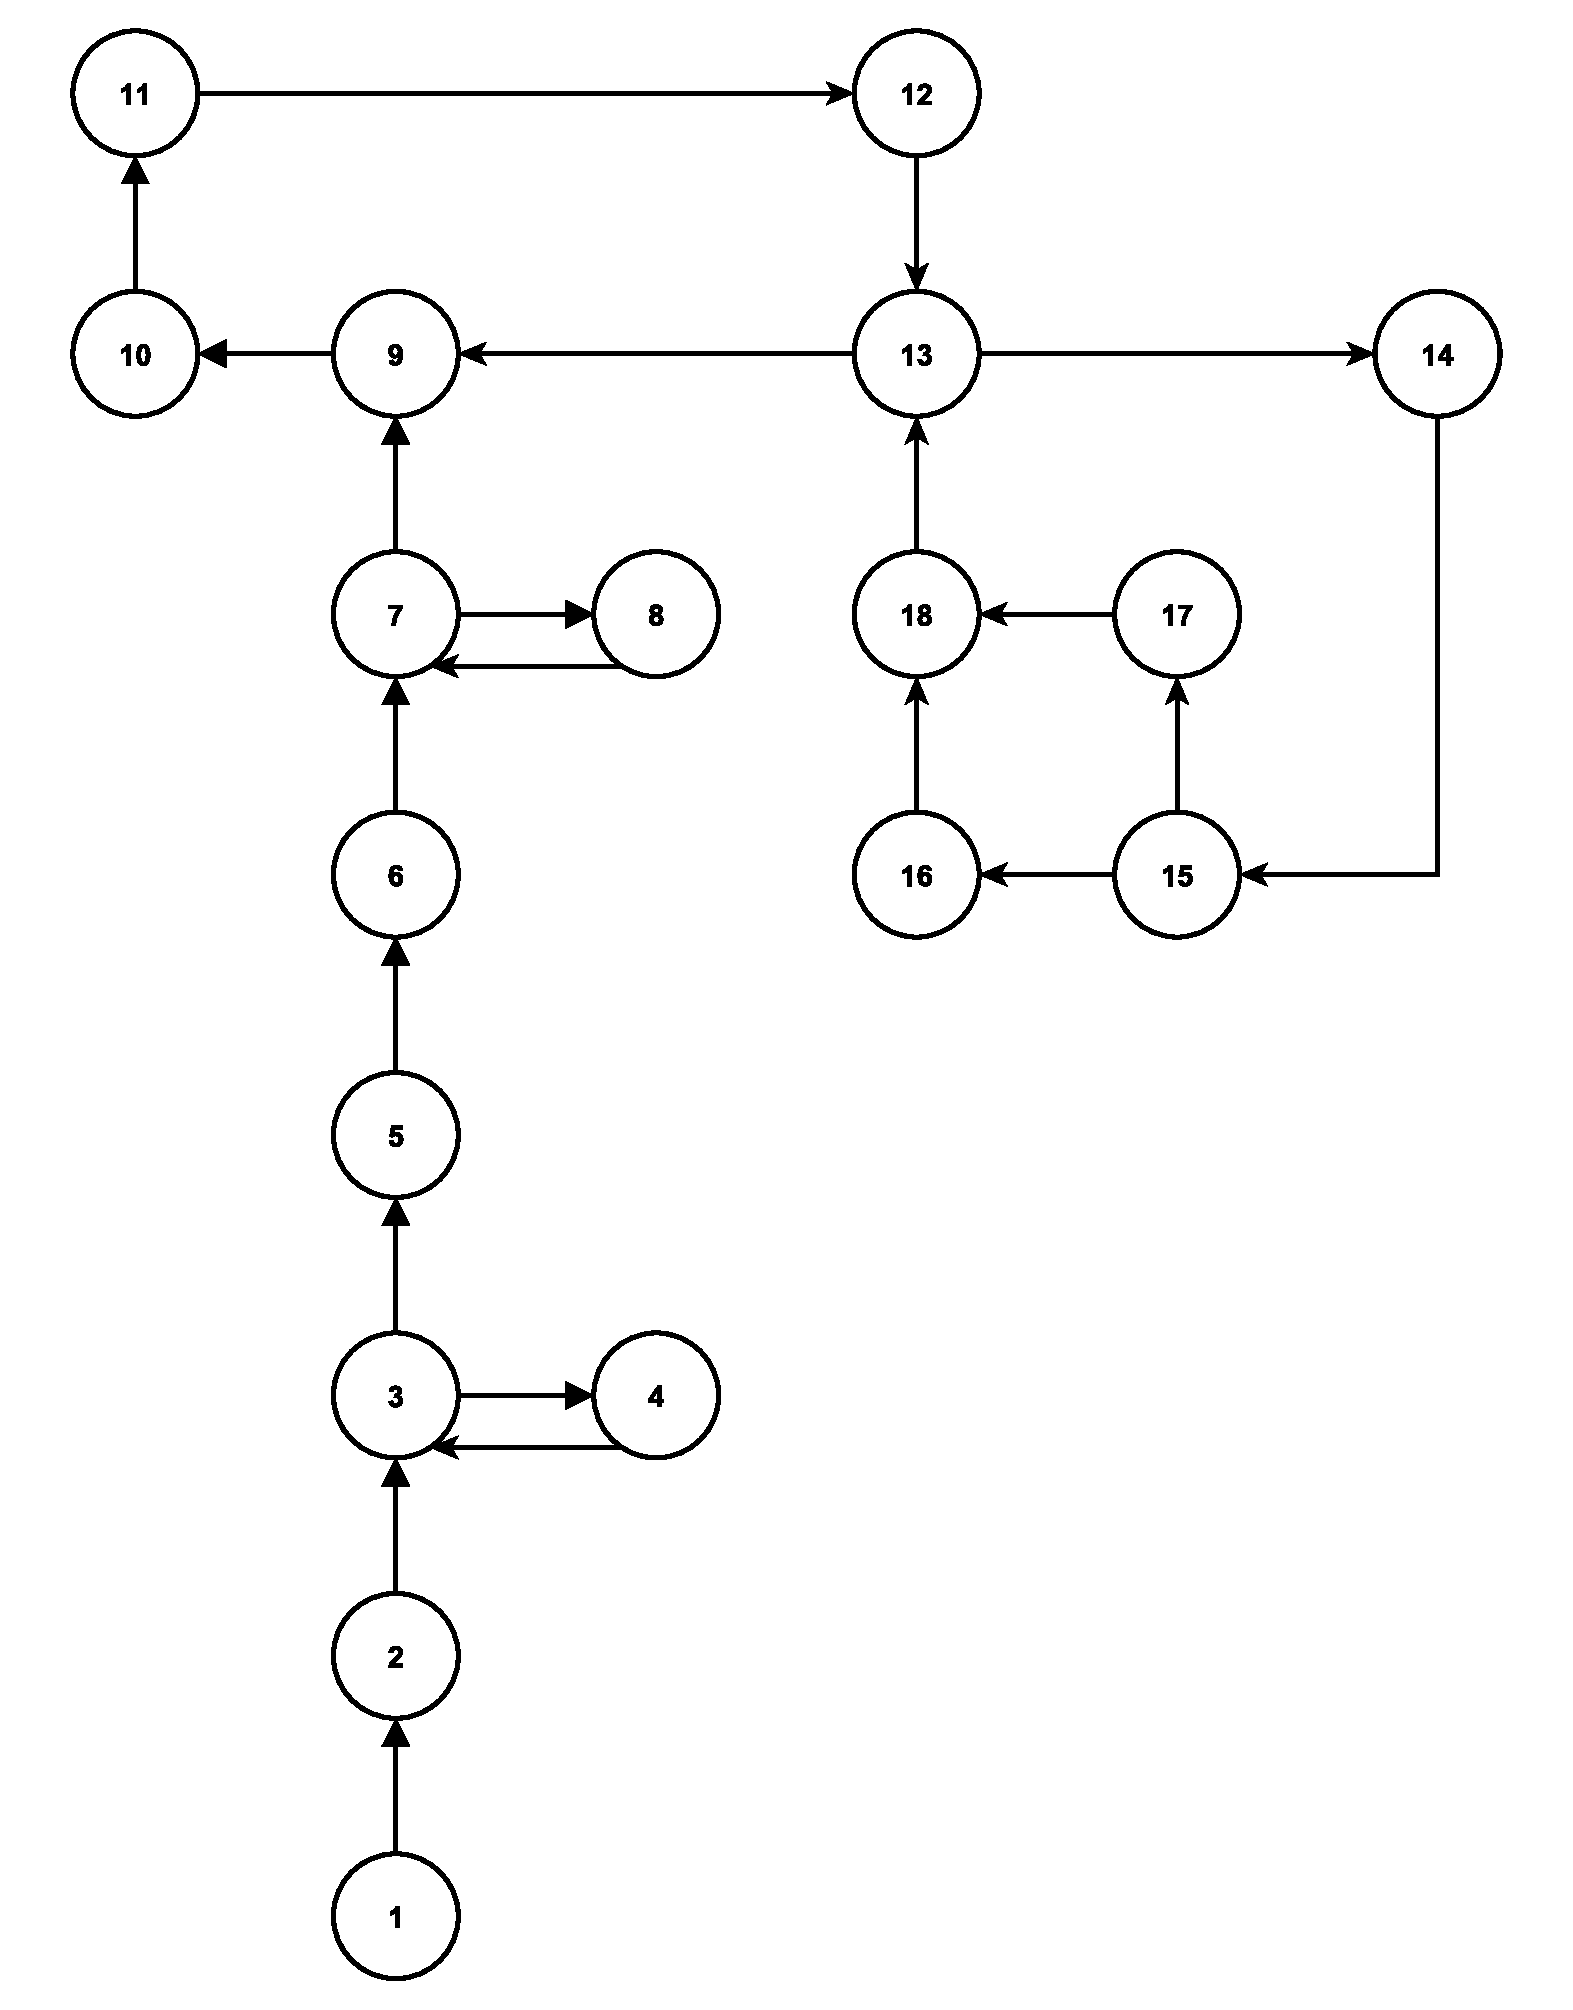
\includegraphics[height=0.4\textheight]{img/граф_управления.pdf}
	\caption{Граф управления}
\end{figure}

\clearpage

\subsection{Информационный граф программы}

\begin{figure}[h]
	\centering
	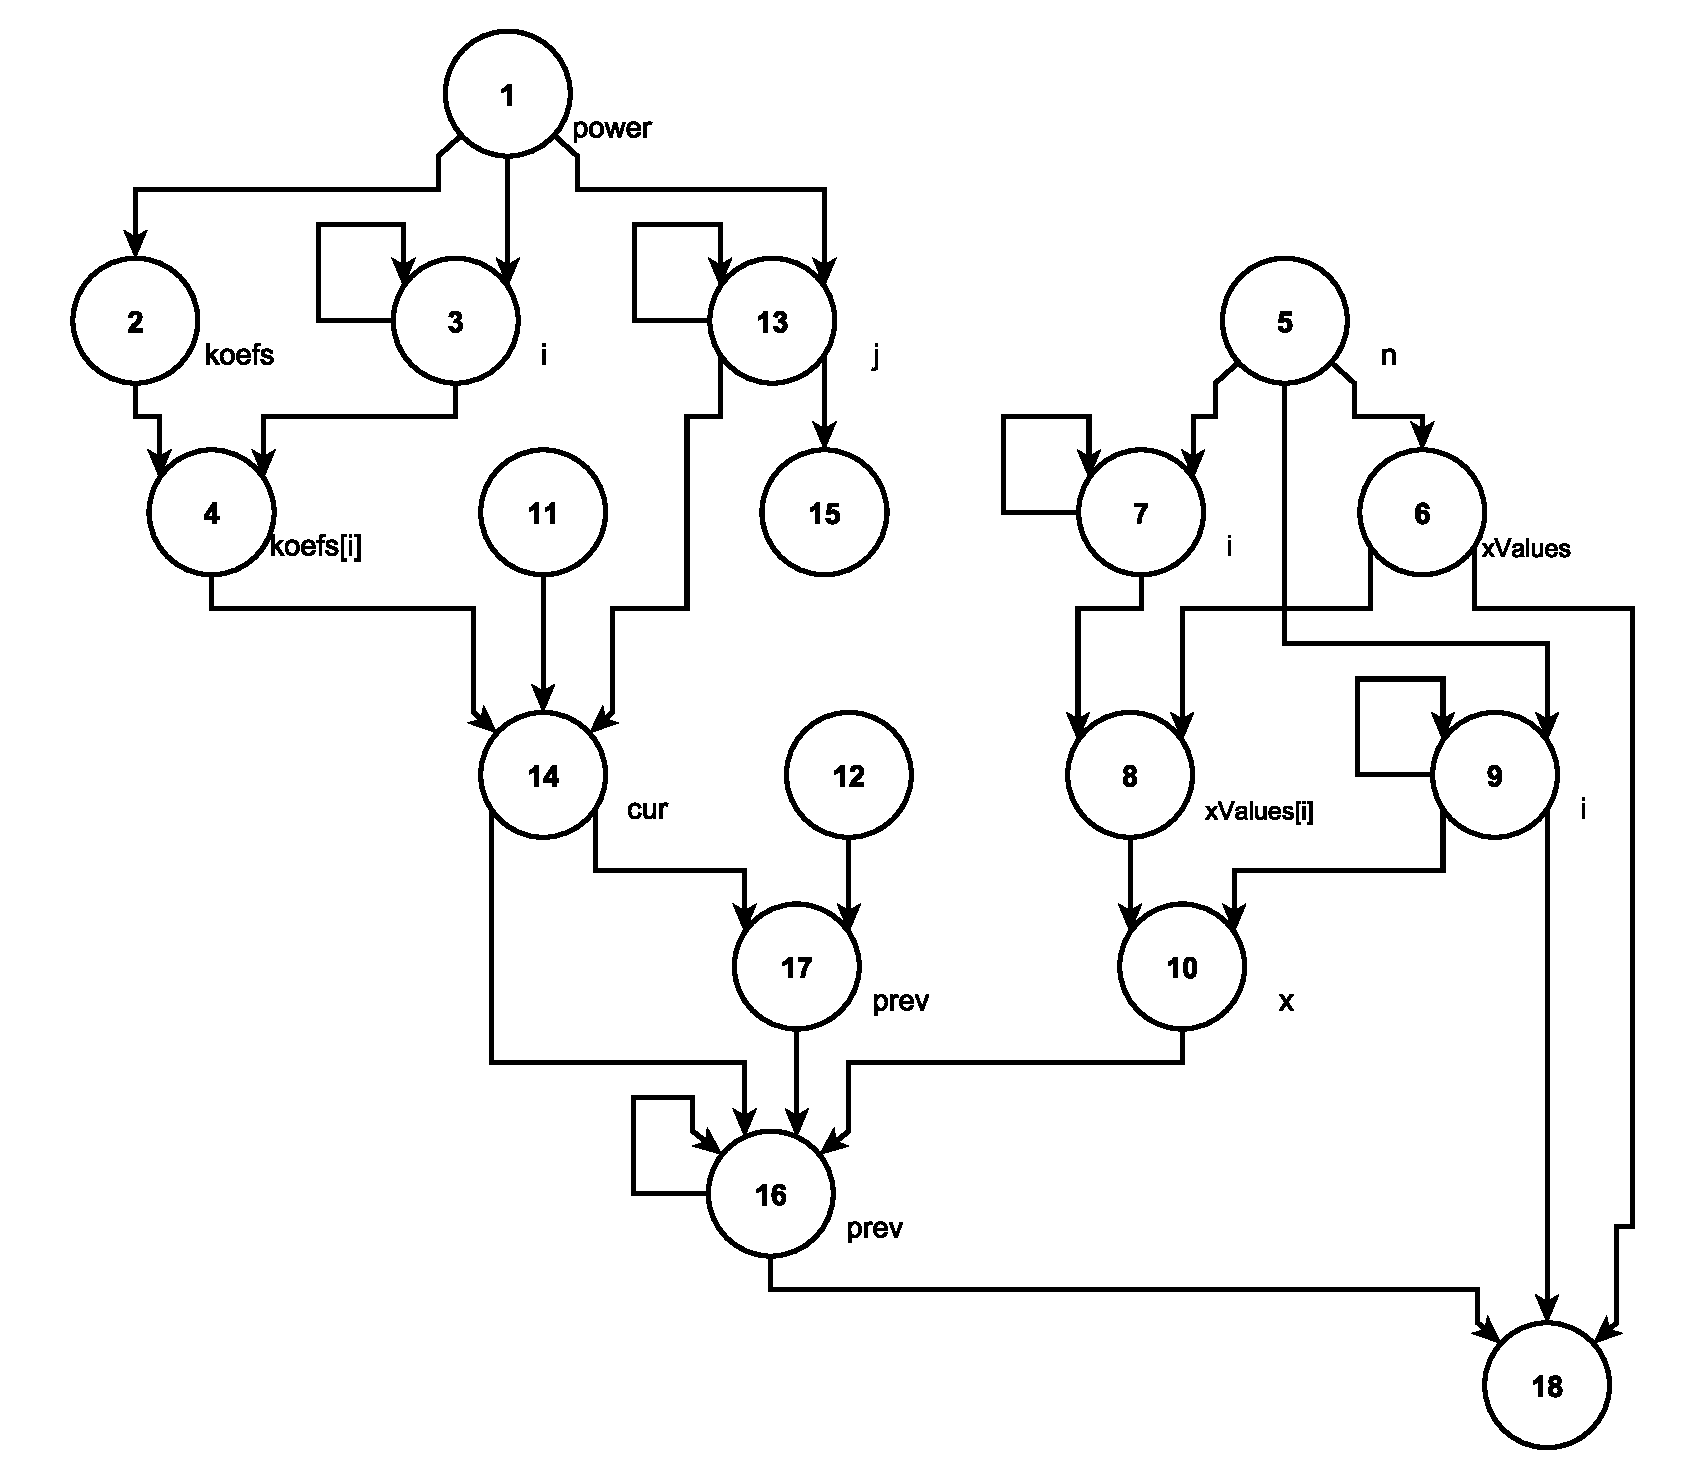
\includegraphics[height=0.6\textheight, page=1]{img/информационный_граф.pdf}
	\caption{Информационный граф}
\end{figure}

\clearpage

\subsection{Операционная история программы}

\begin{figure}[h]
	\centering
	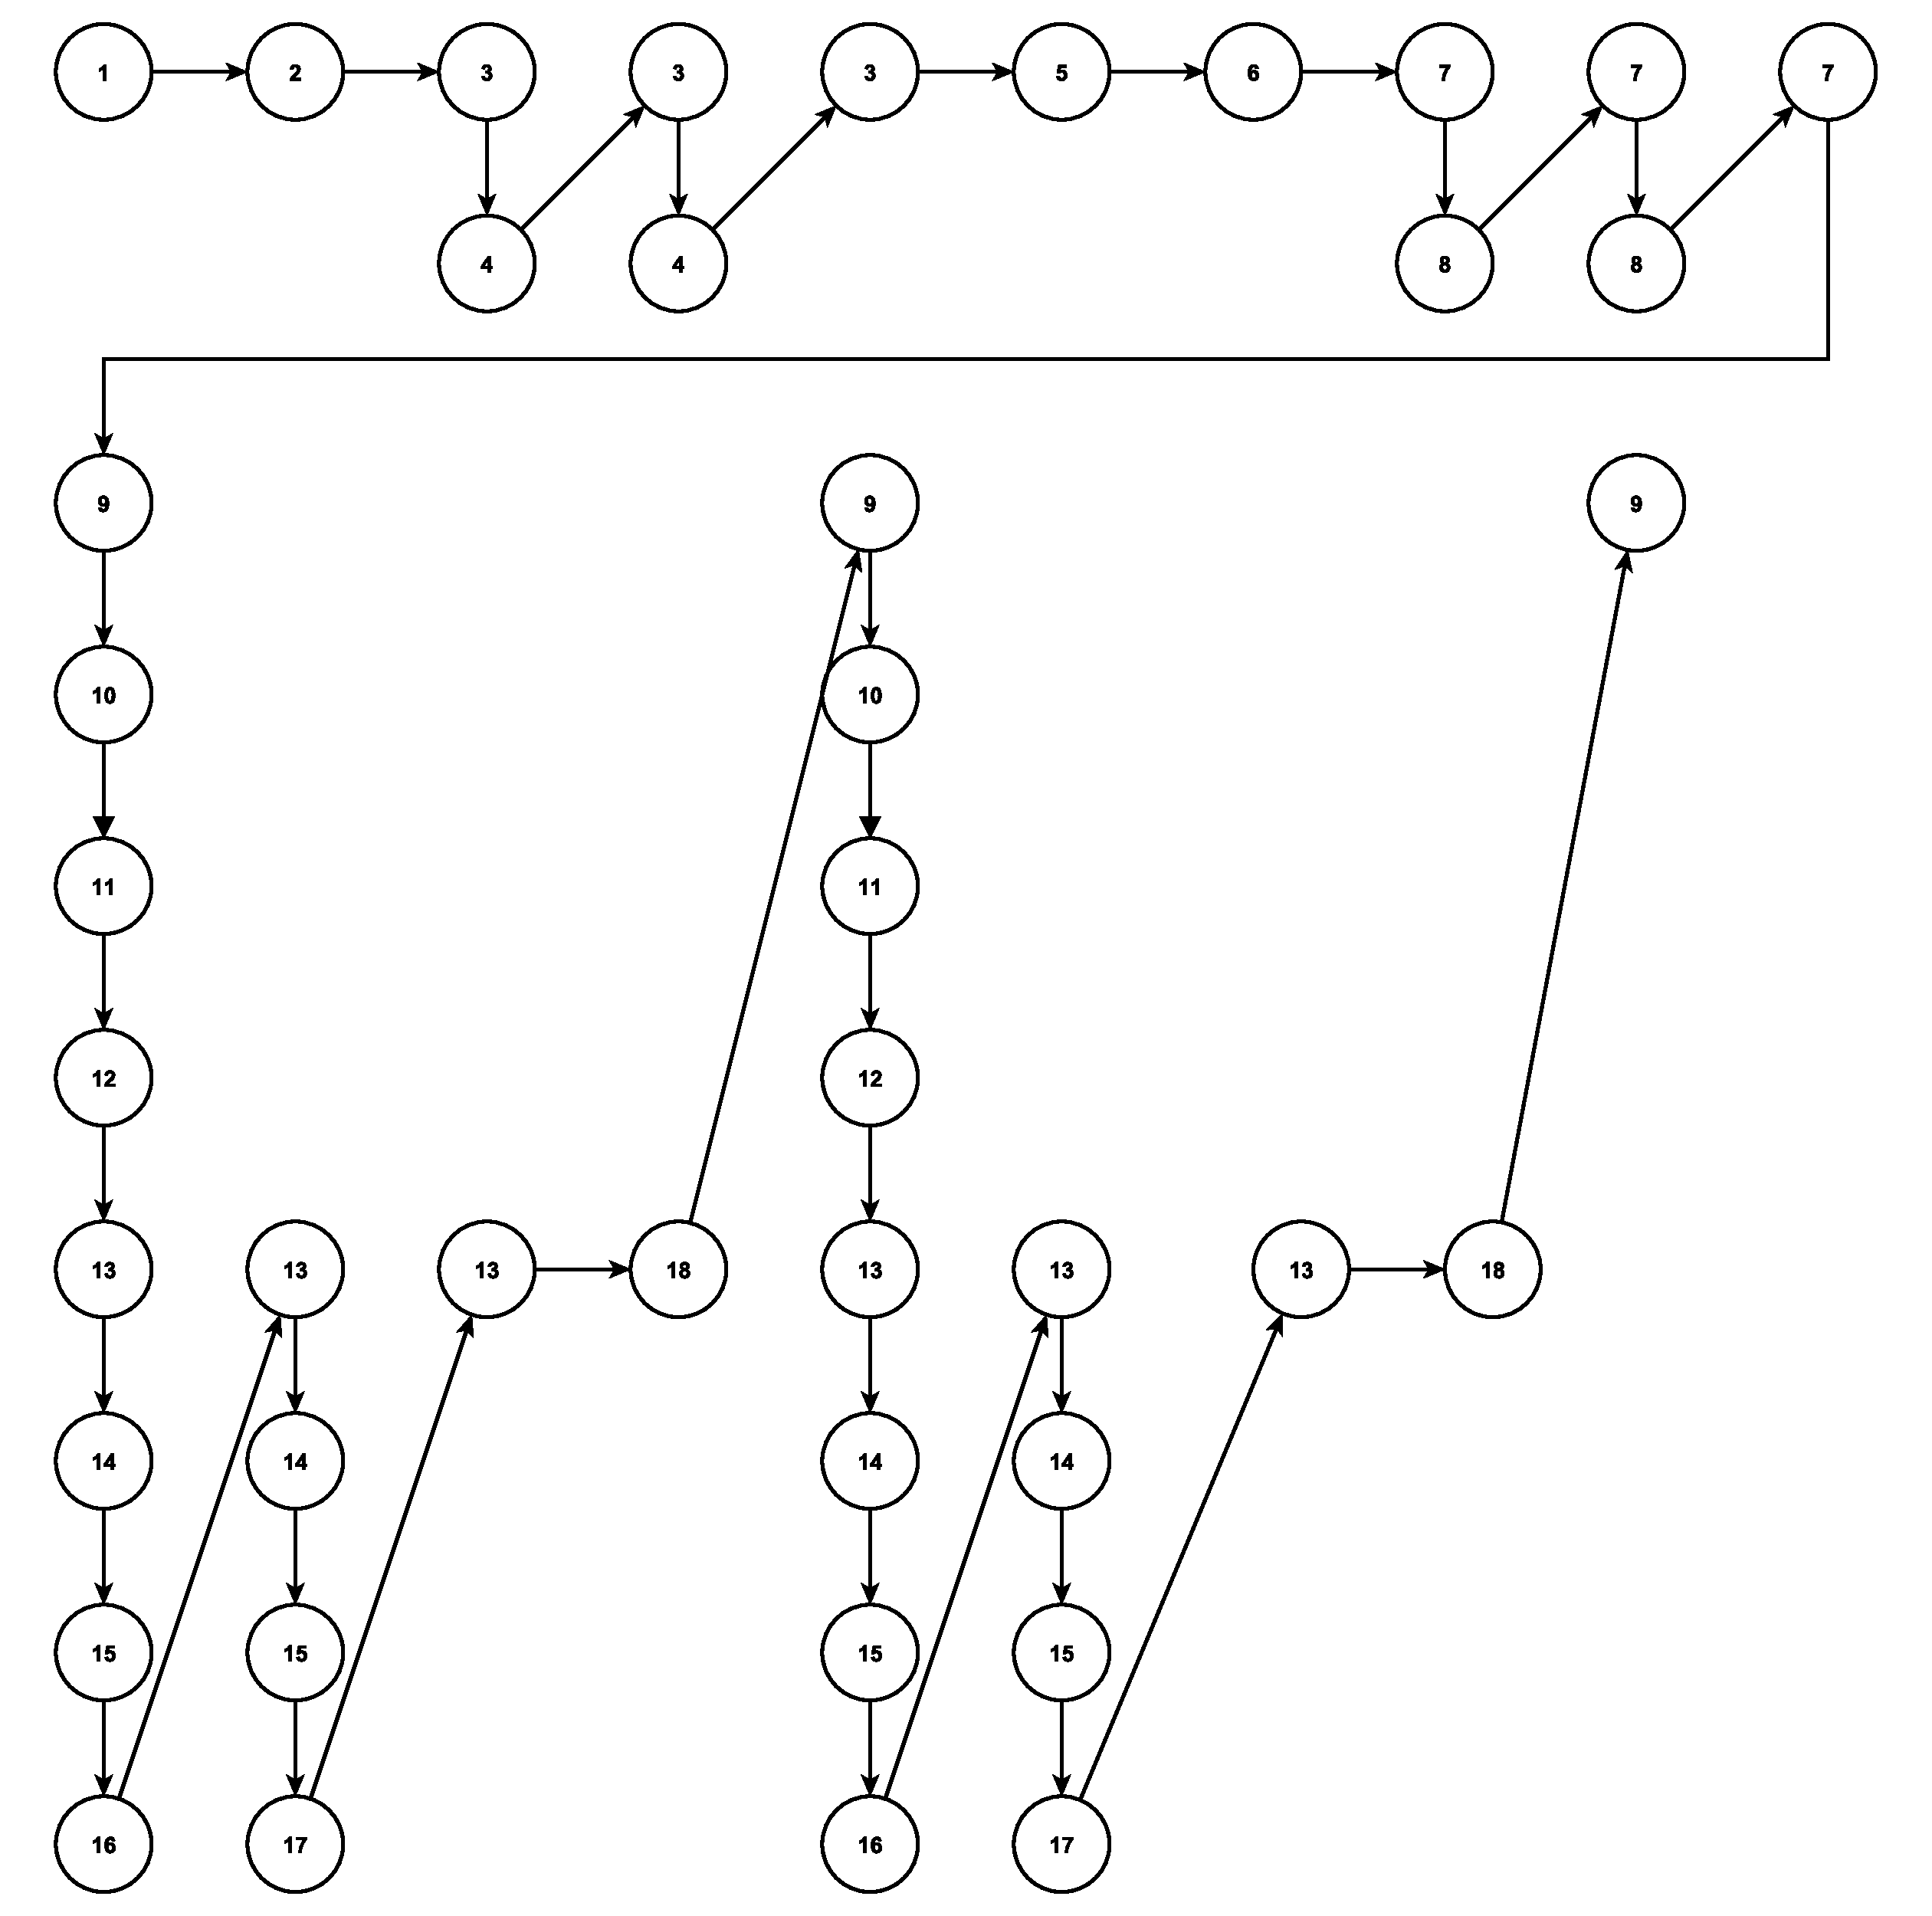
\includegraphics[height=0.7\textheight, page=1]{img/операционная_история.pdf}
	\caption{Операционная история}
\end{figure}

\clearpage

\subsection{Информационная история программы}

\begin{figure}[h]
	\centering
	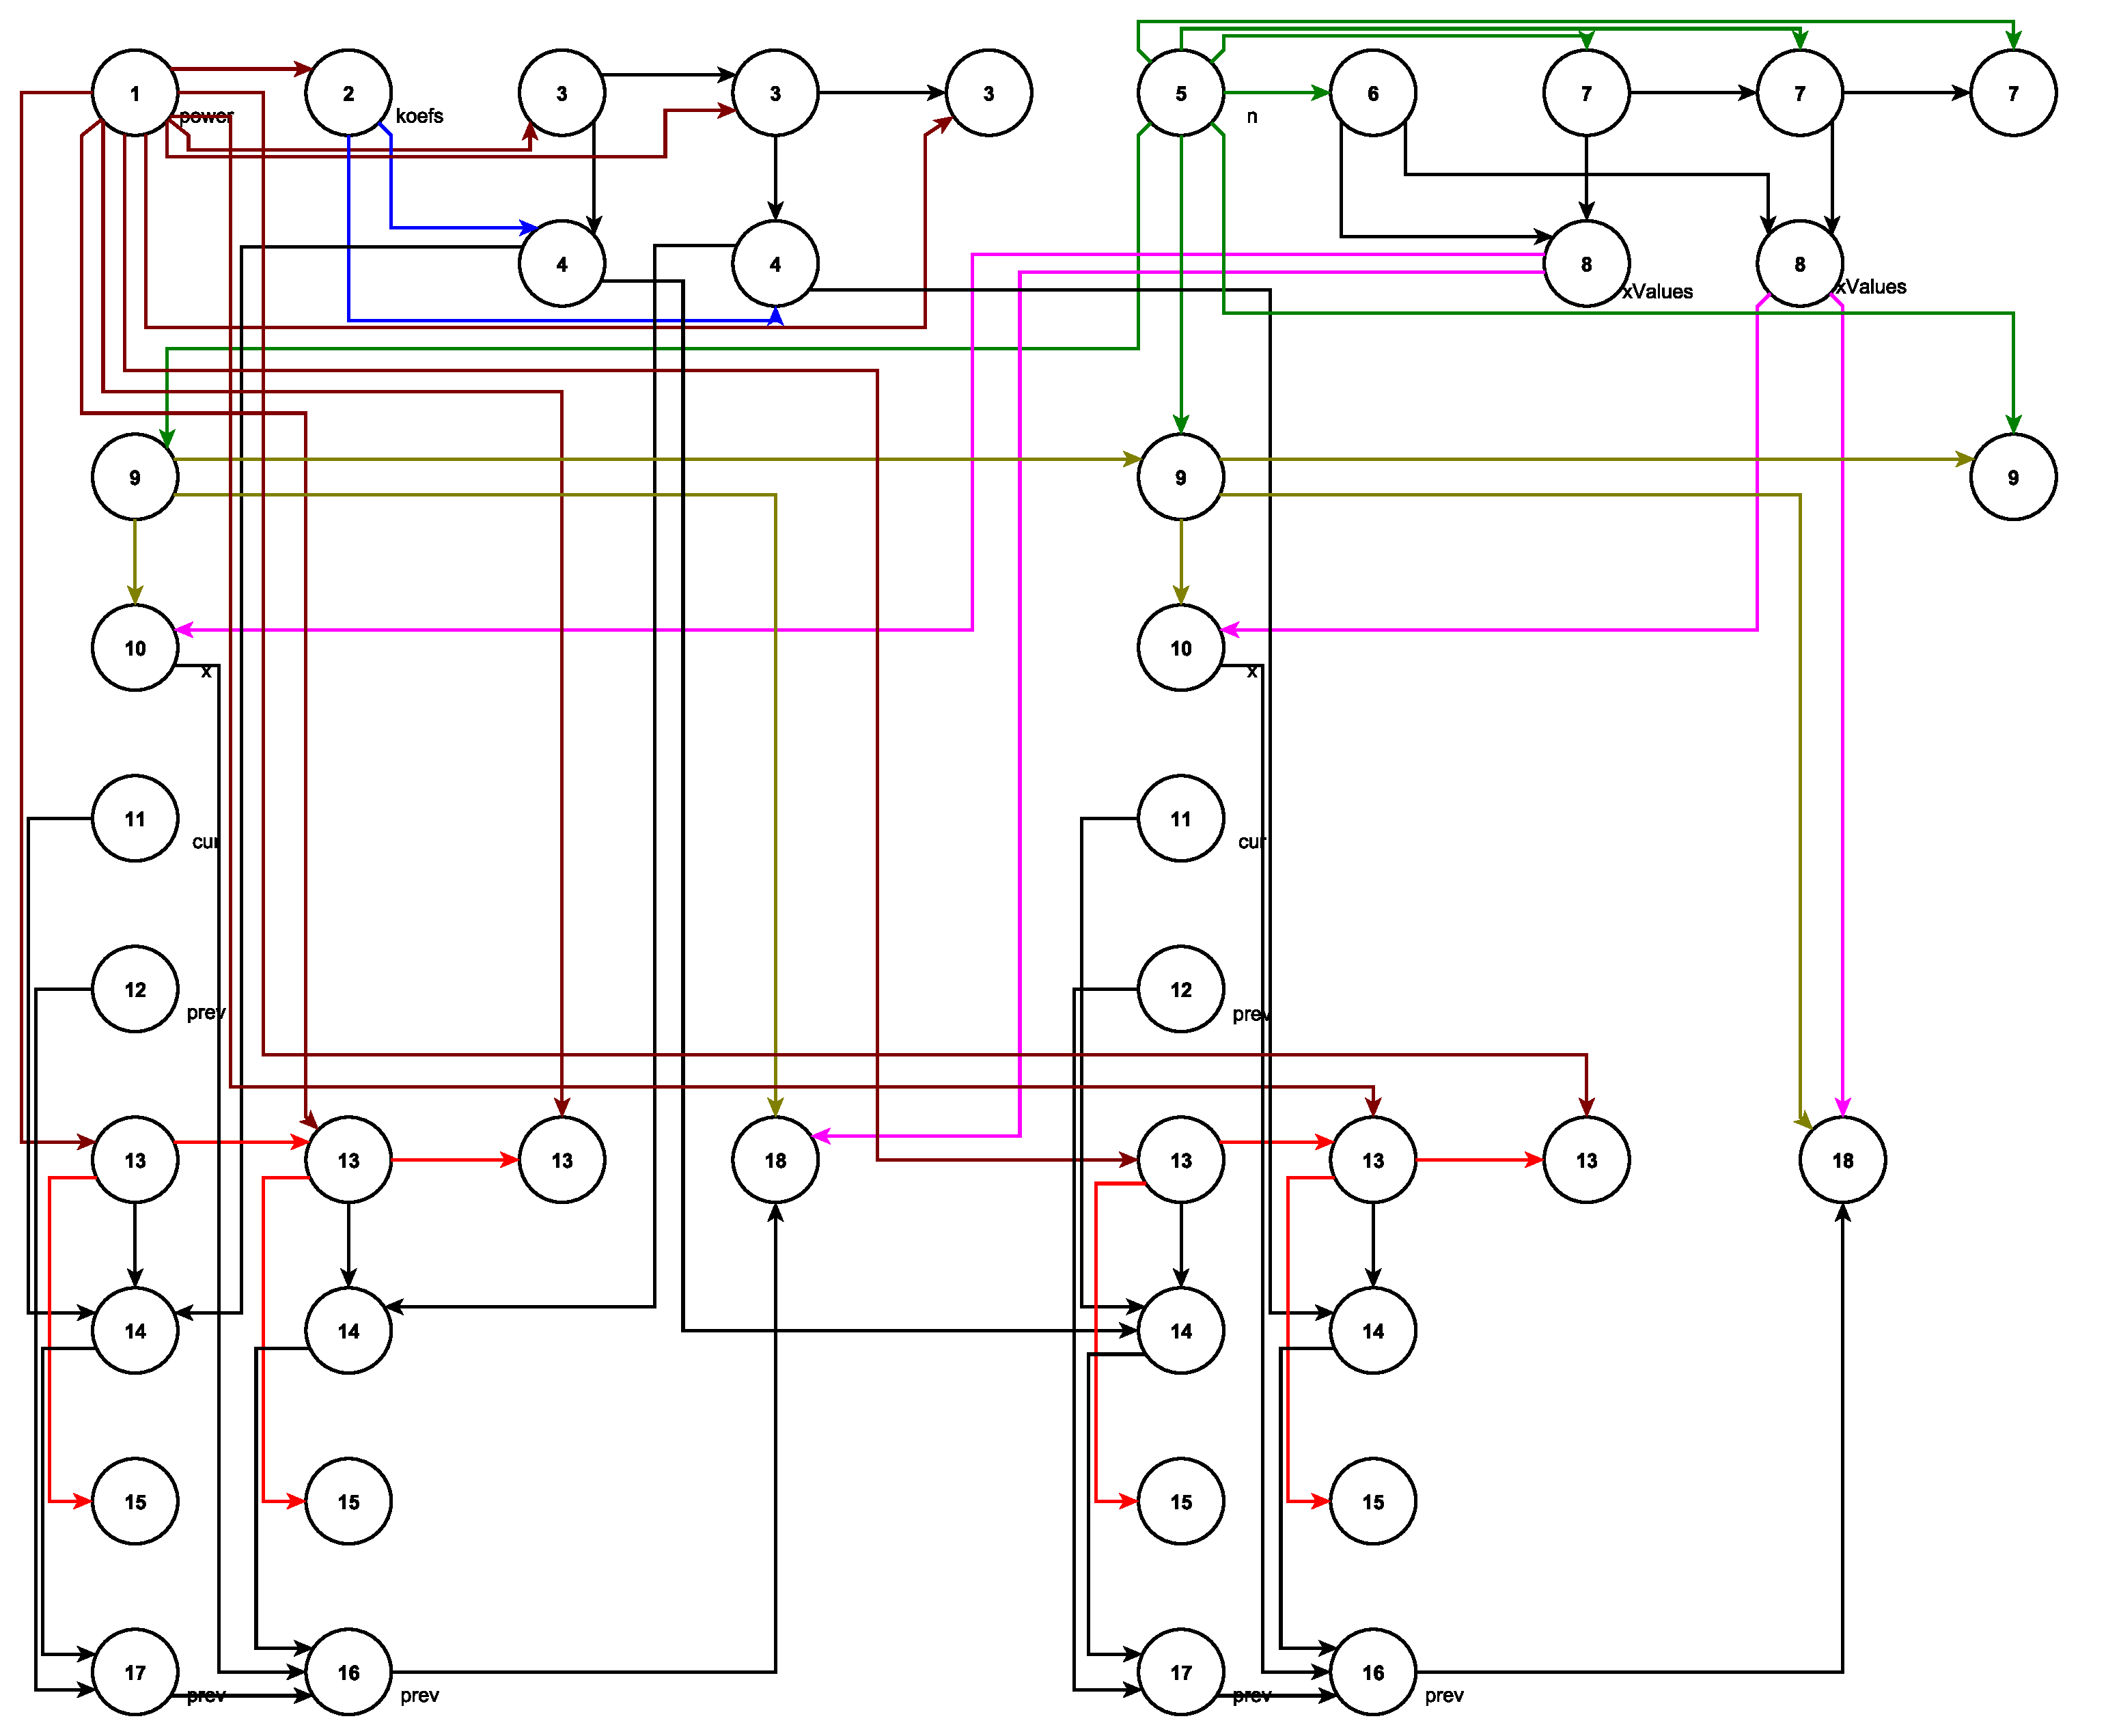
\includegraphics[height=0.7\textheight, page=1]{img/информационная_история.pdf}
	\caption{Информационная история}
\end{figure}

\subsection{Возможность распараллеливания}

Один из способов~--- разделить вычисления на несколько частей, каждую из которых будет обрабатывать свой поток. 
Например, можно разделить массив коэффициентов на равные подмассивы и запустить вычисление частей полинома в отдельных потоках. 
То есть каждый поток будет обрабатывать новый подмасив как отдельный полином.